\chapter{Final Design}
\section{Overview}
This section covers the complete development process including the hardware, gateware, software and mechanical design of the project. It is important to note that the following documentation concentrates only on the final version of the device. Earlier hardware prototypes are not covered due to the lack of relevance.

\subsection{Key Requirements}
The main focus of the development is to design a professional looking, easy to use and eye-catching device for demonstration purposes. The project name \textit{Audio-Beamformer} has been chosen as it is easy to remember and has potential to be seen as a trademark.

The following key requirements have been set:
\begin{itemize}
	\item Single power adapter or power cable (e.g. no need of labor power supplies)
	\item Easy to install (e.g. montage on a camera tripod)
	\item Intuitive to operate via state-of-the-art graphical user interface
	\item Multiple audio streaming sources such as Bluetooth and USB input devices
	\item Great scalability and flexibility of the hardware and software design
\end{itemize}

\subsection{Key Decisions}
In the conceptional phase of the development, several key decisions had to be made. This contains mainly the signal flow and the division between the processing part on the Raspberry Pi and the \acrshort{fpga}. Further, the question had to be evaluated, if a built-in power supply or an external power adapter is preferred. And most importantly, which type of ultrasonic transducer should be used in the design.
In addition, the overall dimension and scale of the final product had to be discussed.
In general, most of these decisions were made according to results of simulations, physical measurements and after extensive discussions.
In the following sections, each part of the project is explained in detail.

\newpage
\section{Mechanical Design}
Blabla




\newpage
\section{Hardware Design}
Blabla

\begin{figure}
	\centering
	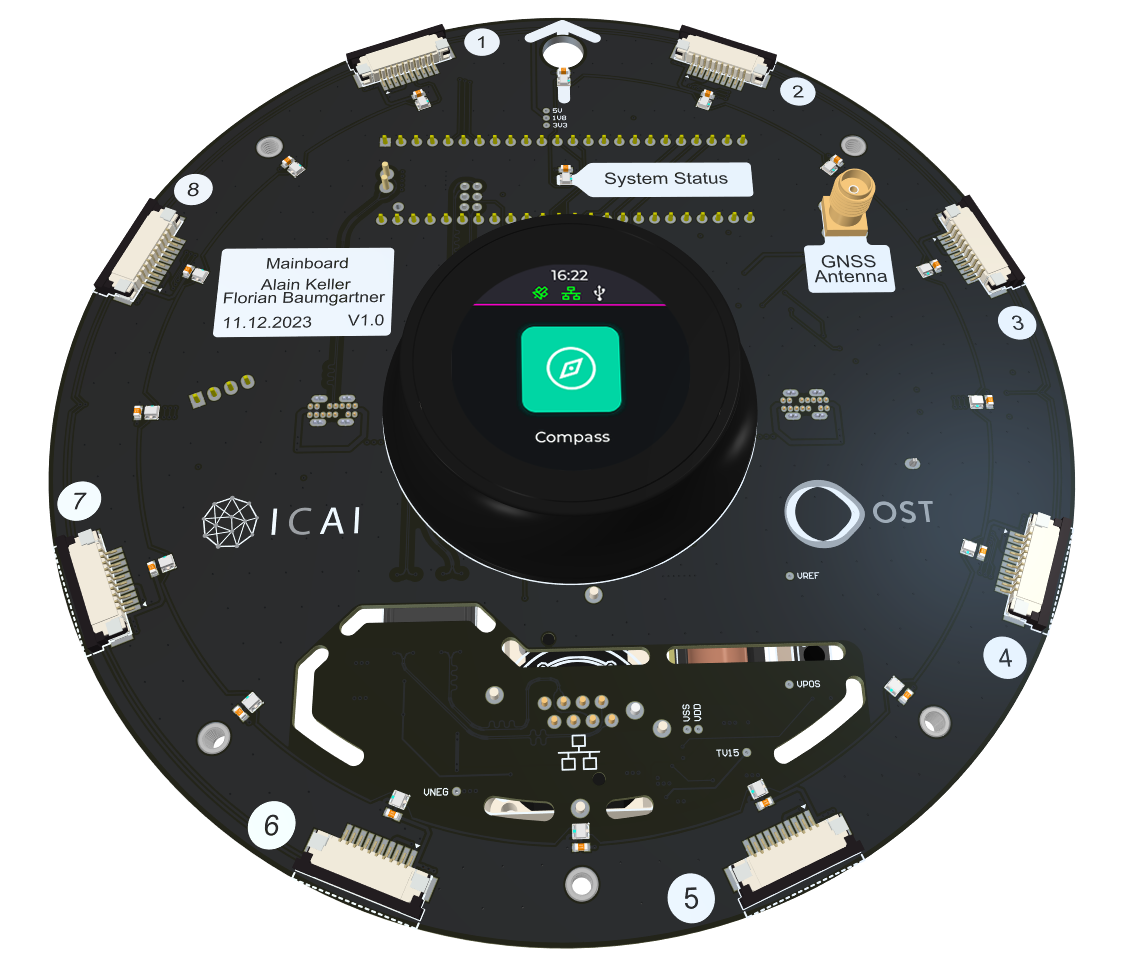
\includegraphics[width=1.0\textwidth]{images/6_design_final/Mainboard_Front_Display.png}
	\caption{Front view of the mainboard}
	\label{fig:mainboard_front}
\end{figure}




\subsection{Block Diagram}

\subsection{Power Supply}

% TODO: Add power supply block diagram

\subsubsection{Power over Ethernet (PoE)}


\subsection{Microcontroller Unit (MCU)}

%  TODO: Write about external PSRAM

\subsection{Audio Input}

\subsubsection{GNSS}

\subsection{Human Machine Interface (HMI)}

%  TODO: Wite about LEDs and Buzzer

\subsubsection{LCD Display}

\subsubsection{RGB LEDs}

\subsection{Sensors}

\subsubsection{Magnetometer \& Accelerometer Sensor}

\subsubsection{Ambient Pressure \& Temperature Sensor}

\subsubsection{Angle Sensor}

\subsection{Printed Circuit Board (PCB)}

\subsubsection{Mainboard}

\subsubsection{Microphone Arms}

\subsubsection{Angle Sensor}

\subsection{Manufacturing}
The PCBs were manufactured and assembled by JLCPCB.
Only a few additional components were soldered by hand, such as the PDM to TDP converters (ADAU7118), the EtherCon connector and the GNSS module (NEO-M8P-2).
It turned out that multiple microphone arm PCBs were faulty (damaged microphones).
This was most likely caused by the soldering process, as the MEMS microphones are very sensitive to heat.

\newpage
\section{Firmware Design}
Blabla

\subsection{Overview}
The firmware is written in C++ and is based on the Arduino framework that has been addopted to the Teensy microcontroller environment.
As an IDE, the VS Code extension PlatfromIO was used, as it provides powerful development tools and a great integration of the Arduino framework.

The firmware is divided into modules running in individual threads, facilitated by TeensyThreads on the Teensy 4.1 microcontroller.
This lightweight multitasking library allows for concurrent execution of multiple threads, optimizing system performance and resource utilization.
TeensyThreads' minimal memory footprint and efficient CPU usage are critical in embedded systems where resources are constrained.


\begin{table}[h]
	\centering
	\begin{tabular}{|l|l|}
		\hline
		Thread                     & Purpose                      \\ \hline
		\texttt{Console Interface} & Handles USB virtual COM-Port \\ \hline
		\texttt{Console Streaming} & Handles queuing of messages  \\ \hline
		\texttt{Utils}             & Updates operation time       \\ \hline
		\texttt{AudioUtils}        & Audio Processing             \\ \hline
		\texttt{GNSS}              & GNSS Data Handling           \\ \hline
		\texttt{HMI}               & LED Control \& RTC           \\ \hline
		\texttt{Buzzer}            & Buzzer Control               \\ \hline
		\texttt{Application}       & Main Application Logic       \\ \hline
		\texttt{Main}              & Main Thread (Background)     \\ \hline
	\end{tabular}
	\caption{Overview of all threads and their purpose}
	\label{tab:threads}
\end{table}


\subsection{Audio Streaming}
The audio streaming module handles the buffering and transmission of the 32 audio channels.
It is based on a TCP server that provides a socket connection on port 6666.
The audio data is transmitted in a lossless 16-bit signed integer format, with a sample rate of 44.1 kHz.

The TCP connection asures a reliable data transmission, which is essential for the audio data.
To provide a low latency audio stream, the audio data is buffered in a circular buffer of 12 MB size.
This allows for a maximum delay of ca. 4.4\,s.

For a continuous audio stream, a tranmission rate of
\begin{equation}
	\frac{32\,\text{channels} \cdot 16\,\text{bit} \cdot 44100\,\text{Hz}}{10^6\,\text{bit/s}} = 22.1184\,\text{Mbit/s}
\end{equation}
is required.
The theoretical maximum transmission rate of 100Base-T Ethernet is 100\,Mbit/s.
However, the maximum transmission rate of the Teensy 4.1 is around 60\,Mbit/s, which is still sufficient for the audio stream.

Due to the maximal TCP packet size of 1460 bytes, the audio data is split into concatenated packets.
A frame consists of 128 interleafed samples (32 channels) and is transmitted in 8 packets.
Each frame starts with a 20-byte header.

\begin{table}[h]
	\centering
	\begin{tabular}{|l|l|l|l|}
		\hline
		\textbf{Byte Offset} & \textbf{Data Format}    & \textbf{Description} & \textbf{Example Value} \\ \hline
		0-7                  & String                  & Magic Sequence       & "HERON666"             \\ \hline
		8-11                 & Integer (Little Endian) & Packet Index         & 12345                  \\ \hline
		12-19                & Integer (Little Endian) & Timestamp (ns)       & 1616929134054668023    \\ \hline
	\end{tabular}
	\caption{Description of the 20-byte Packet Header}
	\label{tab:packet_header}
\end{table}

% TODO: Add frame example diagram
\begin{figure}[h]
	\centering
	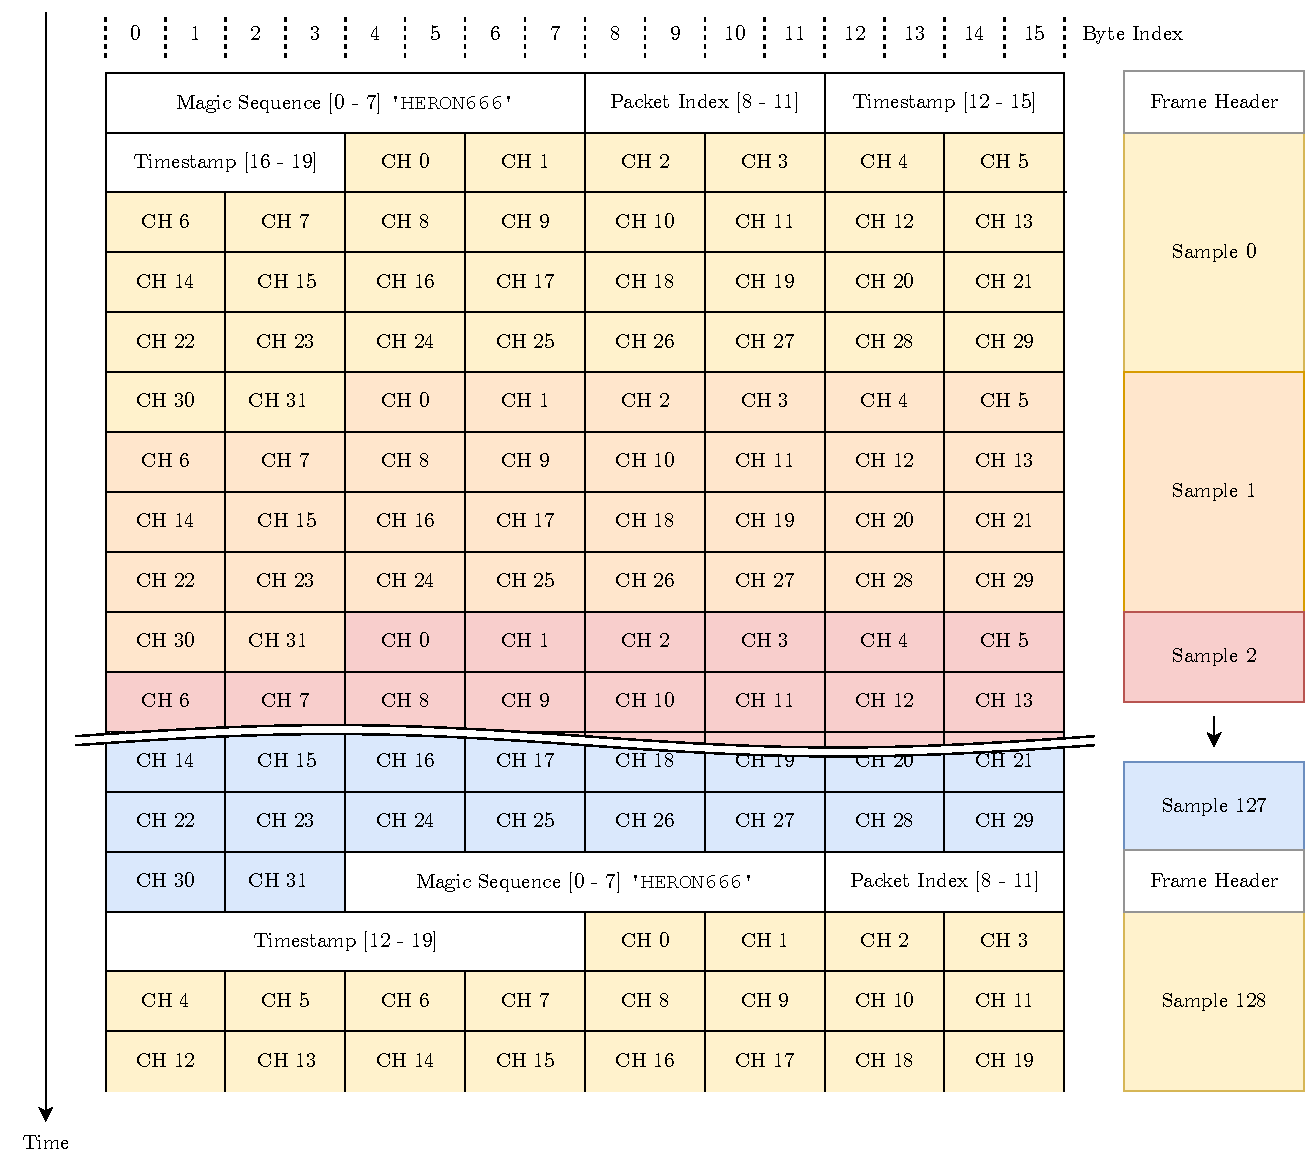
\includegraphics[width=1.0\textwidth]{images/6_design_final/Audio_Stream_Frame.pdf}
	\caption{Example of a Frame with 128 Samples (32 Channels)}
	\label{fig:frame_example}
\end{figure}

\subsubsection{Remote Configuration}
The

\begin{table}[h]
	\tiny
	\centering
	\begin{tabular}{|l|l|l|l|l|}
		\hline
		\textbf{Data Field}         & \textbf{Description}          & \textbf{Data Type} & \textbf{Unit} & \textbf{Example Value} \\ \hline
		device\_firmware\_version   & Firmware Version              & String             & -             & "V0.1"                 \\ \hline
		device\_firmware\_build     & Firmware Build Date           & String             & -             & "240110"               \\ \hline
		device\_cpu\_frequency      & CPU Frequency                 & Integer            & Hz            & 912000000              \\ \hline
		device\_cpu\_temperature    & Current CPU Temperature       & Float              & °C            & 36.5                   \\ \hline
		device\_operating\_time     & Device Operating Time         & Integer            & s             & 15615                  \\ \hline
		device\_system\_warning     & Current System Warning Status & Boolean            & -             & false                  \\ \hline
		ethernet\_mac               & MAC Address                   & String             & -             & "DE:AD:BE:EF:FE:ED"    \\ \hline
		ethernet\_ip                & Current IP Address            & String             & -             & "192.168.1.10"         \\ \hline
		streaming\_state            & Current Streaming State       & Boolean            & -             & true                   \\ \hline
		streaming\_speed            & Current Streaming Speed       & Float              & Mbit/s        & 22.21                  \\ \hline
		streaming\_buffer           & Streaming Buffer Fill Level   & Float              & \%            & 15.1                   \\ \hline
		sensor\_heading             & Device Heading                & Float              & °             & 270.0                  \\ \hline
		sensor\_pitch               & Device Pitch                  & Float              & °             & 5.2                    \\ \hline
		sensor\_roll                & Device Roll                   & Float              & °             & 2.4                    \\ \hline
		sensor\_temperature         & Ambient Temperature           & Float              & °C            & 22.3                   \\ \hline
		sensor\_pressure            & Ambient Pressure              & Float              & hPa           & 1013.2                 \\ \hline
		sensor\_altitude            & Device Altitude               & Float              & m (MSL)       & 434.5                  \\ \hline
		sensor\_angle               & Arm Angle                     & Float              & °             & 45.7                   \\ \hline
		sensor\_magnet\_detected    & Magnet Detection Status       & Boolean            & -             & true                   \\ \hline
		sensor\_magnet\_too\_weak   & Magnet Too Weak Status        & Boolean            & -             & false                  \\ \hline
		sensor\_magnet\_too\_strong & Magnet Too Strong Status      & Boolean            & -             & false                  \\ \hline
		gnss\_latitude              & GNSS Latitude                 & Float              & °             & 40.7128                \\ \hline
		gnss\_longitude             & GNSS Longitude                & Float              & °             & -74.0060               \\ \hline
		gnss\_altitude              & GNSS Altitude                 & Float              & m (MSL)       & 344.8                  \\ \hline
		gnss\_magnetic\_declination & GNSS Magnetic Declination     & Float              & °             & -5.0                   \\ \hline
		gnss\_satelite\_count       & GNSS Satellite Count          & Integer            & -             & 8                      \\ \hline
		gnss\_fix                   & GNSS Fix Status               & Boolean            & -             & true                   \\ \hline
		gnss\_fix\_type             & GNSS Fix Type                 & Integer            & -             & 3                      \\ \hline
		gnss\_time\_valid           & GNSS Time Validity            & Integer            & UNIX (UTC+0)  & 1704921651             \\ \hline
	\end{tabular}
	\caption{Device Data JSON File Fields, Descriptions, Data Types, Units, and Example Values}
	\label{table:device_data_types}
\end{table}


For remote configuration, the client (e.g. a PC) sends a JSON file containing the desired command and its parameters to the device.

\begin{table}[h]
	\tiny
	\centering
	\begin{tabular}{|l|l|l|l|l|}
		\hline
		\textbf{Data Field}    & \textbf{Description}                       & \textbf{Data Type} & \textbf{Unit} & \textbf{Example Value} \\ \hline
		clear\_warning         & Clears the warning status                  & Boolean            & -             & true / false           \\ \hline
		gnss\_coefficient\_xxx & GNSS RTK Coefficient XXX (Not implemented) & Float              & -             & -                      \\ \hline
	\end{tabular}
	\caption{Overview of Received Commands in JSON File}
	\label{tab:received_commands}
\end{table}

\subsection{Sensor Calibration}



\subsection{Grphical User Interface (GUI)}
The GUI provides a user-friendly interface for configuring the device and monitoring its status.
It is based on the LVGL framework.

\subsubsection{Light and Versatile Embedded Graphics Library (LVGL)}
LVGL (Light and Versatile Graphics Library) is a free and open-source graphics library, primarily used for creating embedded GUIs (Graphical User Interfaces).
It's designed to be lightweight, consuming minimal memory and processing power, which is essential in embedded systems where resources are limited.

The decision to use LVGL in conjunction with the NXP GuiGuider, a graphical design tool, enables a rich set of features and enables rapid development.
GuiGuider provides a user-friendly interface for designing GUIs, significantly simplifying the process of creating complex, visually appealing interfaces for embedded systems.
It also provides a code generator, which generates the necessary code to initialize and use the GUI in the firmware.

\subsection{GUI Pages}

\subsubsection{Splash Screen}

\subsubsection{Home Menu}

\subsubsection{System Information}

\subsubsection{Ethernet}

\subsubsection{Ethernet Setup}

\subsubsection{GNSS}

\subsubsection{GNSS Location QR-Code}

\subsubsection{Compass}

\subsubsection{Compass Calibration}

\subsubsection{Arm Angle}

\subsubsection{Arm Angle Calibration}

\subsubsection{Ambient Sensor}

\subsubsection{Settings}

\newpage
\section{Software Design}
Blabla




